\title{Aula 9 - Cifras de bloco}

\author{Prof. Gabriel Rodrigues Caldas de Aquino}

\institute
{
    Instituto de Computação \\
    Universidade Federal do Rio de Janeiro\\
    gabrielaquino@ic.ufrj.br% Your institution for the title page
}
\date{Compilado em: \\ \today} % Date, can be changed to a custom date

%----------------------------------------------------------------------------------------
%    PRESENTATION SLIDES
%----------------------------------------------------------------------------------------



\begin{frame}
    % Print the title page as the first slide
    \titlepage
\end{frame}

\begin{frame}{Cifras de Fluxo vs Cifras de Bloco}
\textbf{Cifras de Fluxo:}
\begin{itemize}
    \item Encriptam dados um \textbf{bit} ou \textbf{byte} por vez.
    \item Exemplos clássicos: Vigenère autochaveada e Vernam.
    \item Ideal: One-time pad (inquebrável se o fluxo de chaves for verdadeiramente aleatório).
    \item Limitação prática: o fluxo de chaves precisa ser compartilhado previamente via canal seguro.
    \item Solução prática: gerar o fluxo de bits algoritmicamente, controlado por chave, garantindo que partes futuras do fluxo sejam imprevisíveis.
\end{itemize}

\medskip
\textbf{Cifras de Bloco:}
\begin{itemize}
    \item Tratam um \textbf{bloco} de texto claro como um todo, normalmente de 64 ou 128 bits.
    \item Usuários compartilham uma chave simétrica.
    \item Modos de operação permitem uso semelhante ao das cifras de fluxo.
    \item Mais analisadas e amplamente utilizadas em aplicações de criptografia simétrica.
\end{itemize}
\end{frame}

\begin{frame}{Cifra de fluxo vs. Cifra de bloco}

\centering
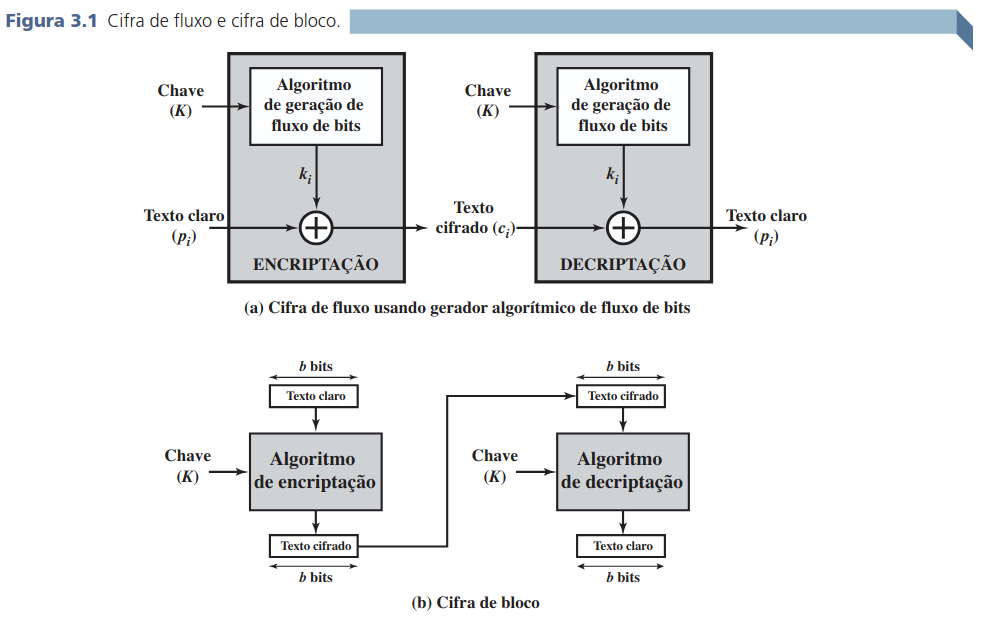
\includegraphics[width=0.9\linewidth]{Figuras/cifra-de-bloco-cifra-de-fluxo.png}


\end{frame}


\begin{frame}{Confusão e Difusão segundo Claude Shannon}
\textbf{Contexto histórico:}
\begin{itemize}
    \item Claude Shannon desenvolveu a ideia de \textbf{cifras de produto}, alternando funções de confusão e difusão \cite{SHAN49}.
    \item A estrutura da \textbf{cifra de Feistel}, baseada na proposta de Shannon de 1945, é utilizada em muitas cifras de bloco simétricas atuais.
\end{itemize}

\medskip
\textbf{Conceitos de Shannon:}
\begin{itemize}
    \item \textbf{Difusão}: espalhar a influência de cada bit do texto claro por muitos bits do texto cifrado, dificultando deduções estatísticas.
    \item \textbf{Confusão}: tornar a relação entre chave e texto cifrado complexa, de modo que conhecer parte da saída não revele informações sobre a chave.
\end{itemize}

\medskip
\textbf{Objetivo:} impedir criptoanálise baseada em estatísticas do texto claro, como frequências de letras ou palavras prováveis.
\end{frame}

\begin{frame}{Difusão em Criptografia}
A difusão busca dissociar a estrutura estatística do texto claro das estatísticas do texto cifrado.  

\medskip
\textbf{Princípio:} Cada dígito do texto claro deve afetar muitos dígitos do texto cifrado, espalhando a informação.  

\medskip
\textbf{Exemplo matemático:} Para uma mensagem $M = m_1, m_2, m_3, \dots$:
\[
y_n = \left( \sum_{i=1}^{k} m_{n+i} \right) \bmod 26
\]
onde $k$ letras sucessivas do texto claro influenciam cada letra do texto cifrado.  

\medskip
\textbf{Efeito:} 
\begin{itemize}
    \item Frequências de letras e dígrafos no texto cifrado se aproximam de uma distribuição uniforme.  
    \item Em cifras de bloco binárias, difusão é alcançada por permutações seguidas de funções de transformação, garantindo que bits de diferentes posições contribuam para cada bit cifrado.
\end{itemize}
\end{frame}

\begin{frame}{Difusão e Confusão em Cifras de Bloco}
Cada cifra de bloco transforma um bloco de texto claro em texto cifrado, dependendo da chave.  

\medskip
\textbf{Difusão:} 
\begin{itemize}
    \item Complica o relacionamento estatístico entre o texto claro e o texto cifrado.  
    \item Faz com que cada bit do texto claro influencie muitos bits do texto cifrado.  
    \item Frustra tentativas de deduzir padrões no texto claro.  
\end{itemize}

\medskip
\textbf{Confusão:} 
\begin{itemize}
    \item Complica o relacionamento entre o texto cifrado e a chave de encriptação.  
    \item Utiliza funções de substituição complexas para dificultar a descoberta da chave.  
    \item Funções lineares simples resultariam em pouca confusão e vulnerabilidade.  
\end{itemize}
\end{frame}

\begin{frame}{Cifra de Feistel}

\centering
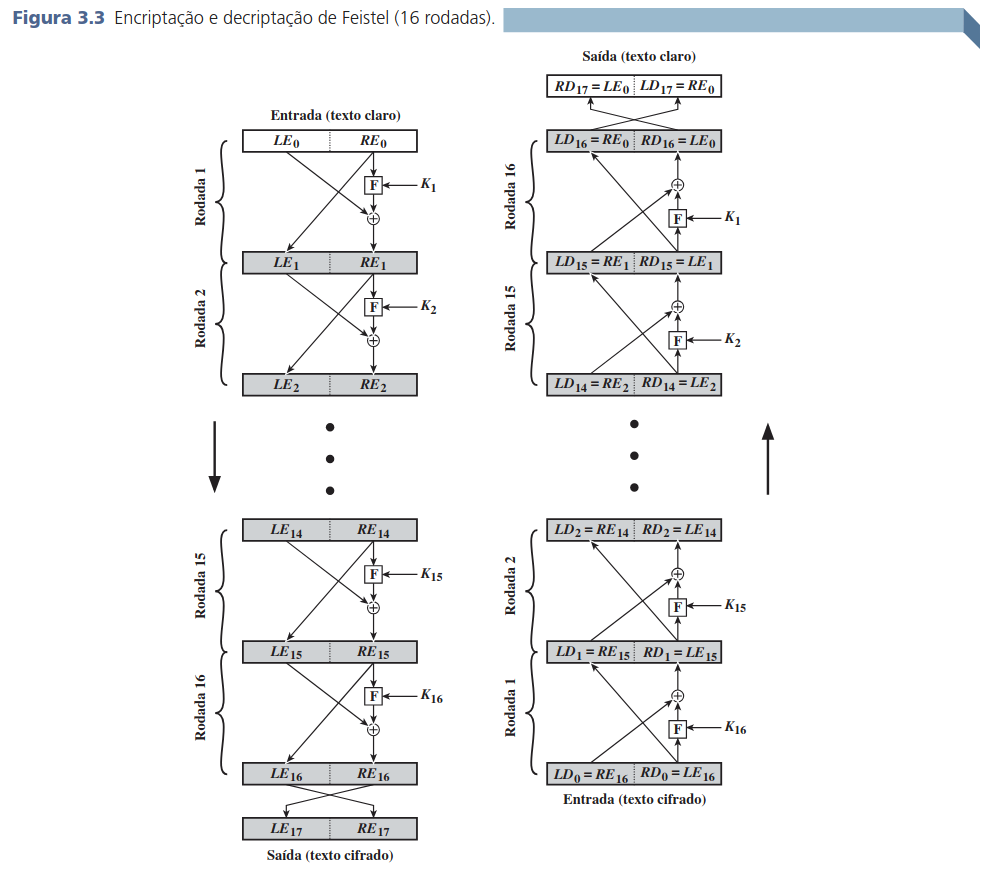
\includegraphics[width=0.6\linewidth]{Figuras/cifra-de-feistel.png}


\end{frame}

\begin{frame}{Estrutura da Cifra de Feistel}
A estrutura de Feistel permite criar cifras de bloco seguras a partir de funções de encriptação simples.

\medskip
\textbf{Descrição:}
\begin{itemize}
    \item Entrada: bloco de texto claro de 2w bits e chave K.
    \item O bloco é dividido em duas metades: $L_0$ e $R_0$.
    \item Os dados passam por $n$ rodadas de processamento.
    \item Cada rodada $i$ recebe $L_{i-1}$, $R_{i-1}$ e uma subchave $K_i$ derivada de $K$.
    \item As subchaves $K_i$ são normalmente diferentes entre si e da chave original.
    \item Após $n$ rodadas, as metades são combinadas para gerar o bloco cifrado.
\end{itemize}

\medskip
\textbf{Exemplo:} 16 rodadas, mas qualquer número de rodadas pode ser implementado.
\end{frame}

\begin{frame}{Rodadas da Cifra de Feistel}
Todas as rodadas têm a mesma estrutura básica:

\medskip
\textbf{Processamento em cada rodada:}
\begin{enumerate}
    \item Aplica-se uma função de substituição $F$ à metade direita dos dados $R_{i-1}$, parametrizada pela subchave $K_i$.
    \item Realiza-se a operação XOR entre a saída de $F$ e a metade esquerda $L_{i-1}$:
    \[
        L_i = L_{i-1} \oplus F(R_{i-1}, K_i)
    \]
    \item Executa-se a permutação trocando as metades:
    \[
        R_i = R_{i-1}, \quad L_i \leftrightarrow R_i
    \]
\end{enumerate}

\medskip
\textbf{Observações:}
\begin{itemize}
    \item $F$ é uma função de $w$ bits de $R_{i-1}$ e $y$ bits de $K_i$, produzindo $w$ bits de saída.
    \item Estrutura geral é repetida em todas as rodadas, formando uma rede de substituição-permutação (SPN) como proposta por Shannon.
\end{itemize}
\end{frame}

\begin{frame}{Fatores que influenciam a segurança da cifra de Feistel}
A execução de uma rede de Feistel depende de diversos parâmetros de projeto, sendo um dos principais:

\medskip
\textbf{Tamanho de bloco:}
\begin{itemize}
    \item Blocos maiores proporcionam maior segurança, mantendo os demais fatores constantes.
    \item Blocos maiores reduzem a velocidade de encriptação/decriptação para um dado algoritmo.
    \item Maior segurança é obtida por meio de maior difusão.
    \item Tradicionalmente, o tamanho de bloco de 64 bits era considerado adequado para cifras de bloco.
    \item O AES moderno utiliza tamanho de bloco de 128 bits.
\end{itemize}
\end{frame}

\begin{frame}{Fatores que influenciam a segurança da cifra de Feistel}
\begin{itemize}
    \item \textbf{Tamanho da chave:} 
    \begin{itemize}
        \item Chave maior $\Rightarrow$ maior resistência a ataques de força bruta e maior confusão.
        \item Impacto: pode reduzir a velocidade de encriptação/decriptação.
        \item 64 bits ou menos: inseguros.
        \item 128 bits: tornou-se padrão comum.
    \end{itemize}

    \item \textbf{Número de rodadas:} 
    \begin{itemize}
        \item 1 rodada: segurança inadequada.
        \item 16 rodadas: valor típico que garante segurança aceitável.
    \end{itemize}

    \item \textbf{Algoritmo de geração de subchaves:} 
    \begin{itemize}
        \item Quanto mais complexo, mais difícil a criptoanálise.
    \end{itemize}

    \item \textbf{Função F:} 
    \begin{itemize}
        \item Função mais complexa $\Rightarrow$ maior resistência a ataques.
    \end{itemize}
\end{itemize}
\end{frame}

\begin{frame}{Considerações adicionais no projeto da cifra de Feistel}
\begin{itemize}
    \item \textbf{Encriptação/Decriptação rápidas em software:}  
    \begin{itemize}
        \item Muitas vezes a implementação ocorre em software, não em hardware.  
        \item Desempenho do algoritmo passa a ser um fator crítico.  
    \end{itemize}

    \item \textbf{Facilidade de análise:}  
    \begin{itemize}
        \item Algoritmos claros e concisos são mais fáceis de avaliar contra ataques.  
        \item Transparência aumenta a confiança na robustez criptográfica.  
        \item Exemplo: o DES não possui estrutura de fácil análise.  
    \end{itemize}
\end{itemize}
\end{frame}
\begin{frame}{Algoritmo de Decriptação de Feistel}
    O processo de decriptação com uma cifra de Feistel é basicamente o mesmo da encriptação.  
    A regra é a seguinte: use o texto cifrado como entrada para o algoritmo, mas aplique as subchaves \(K_i\) em ordem reversa.  

    \vspace{0.5cm}
    Ou seja: 
    \begin{itemize}
        \item Use \(K_n\) na primeira rodada, \(K_{n-1}\) na segunda, \dots, até \(K_1\) na última rodada.
    \end{itemize}

    \vspace{0.3cm}
    \textbf{Observação:} Isso permite que o mesmo algoritmo seja usado tanto para encriptação quanto para decriptação.
\end{frame}

\begin{frame}{Validação do Algoritmo de Feistel com Ordem de Chaves Invertida}

Observando a última rodada de encriptação da Cifra de Feistel e a primeira rodada da decriptação
\begin{figure}
    \centering
    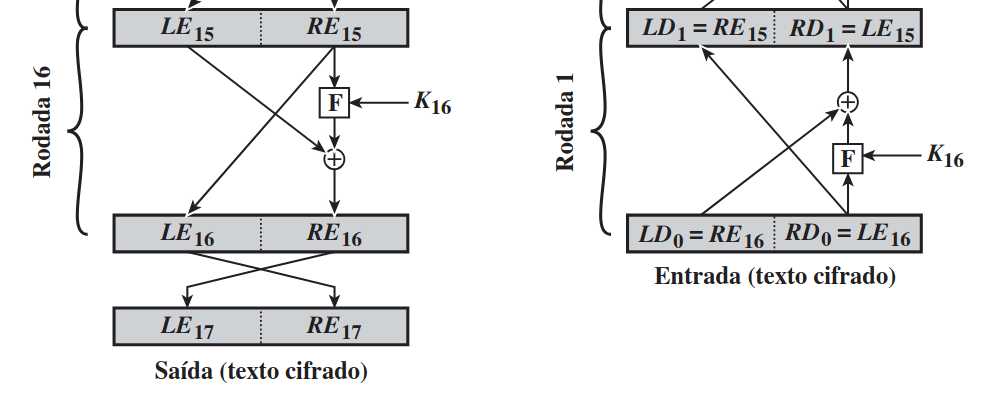
\includegraphics[width=0.5\linewidth]{Figuras/ultima-milha-feistel.png}

\end{figure}

E sabendo que a  operação lógica ou-exclusivo  tem as
seguintes propriedades:

\begin{figure}
    \centering
    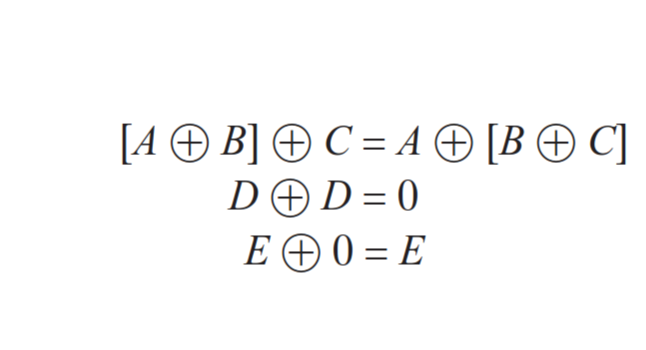
\includegraphics[width=0.4\linewidth]{Figuras/propriedades-xor-feistel.png}

\end{figure}

\end{frame}

\begin{frame}{Validação do Algoritmo de Feistel com Ordem de Chaves Invertida}

Temos:
\begin{figure}
    \centering
    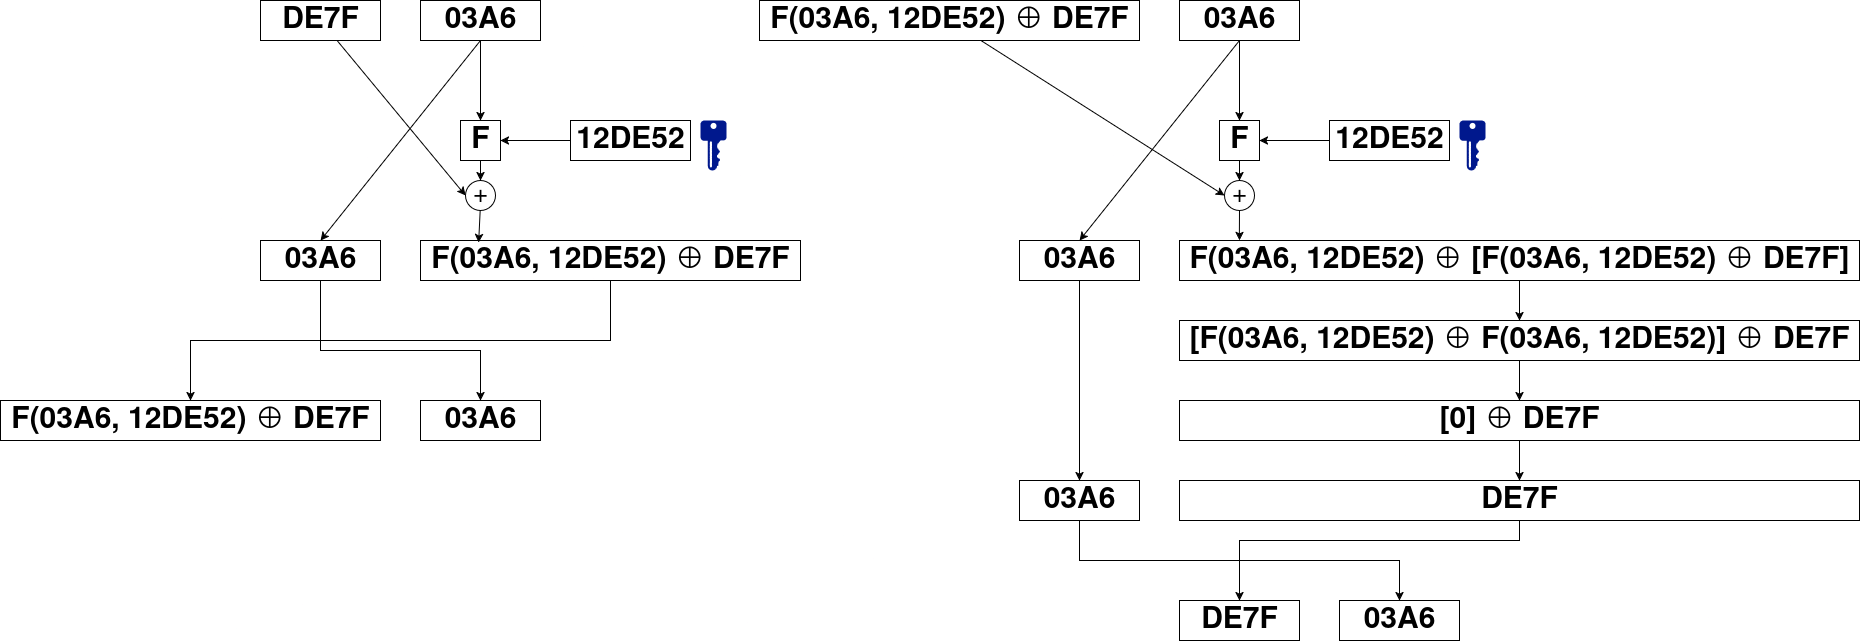
\includegraphics[width=0.9\linewidth]{Figuras/feistel.png}

\end{figure}



\end{frame}

\begin{frame}{Resumindo}

Temos:
\begin{figure}
    \centering
    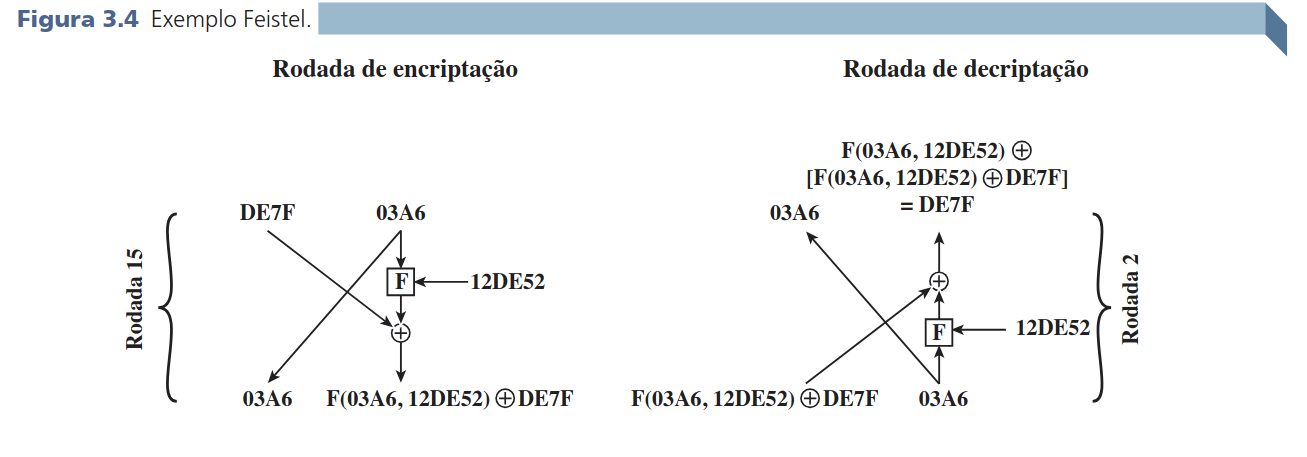
\includegraphics[width=0.9\linewidth]{Figuras/feistel-resumo-livro.png}

\end{figure}



\end{frame}

\begin{frame}{Data Encryption Standard (DES)}
    Até a introdução do \textbf{Advanced Encryption Standard (AES)} em 2001, o DES era o esquema de encriptação mais utilizado.

    \vspace{0.3cm}
    \textbf{Histórico:}
    \begin{itemize}
        \item Adotado em 1977 pelo \textbf{NIST}.
        \item Também conhecido como \textbf{Data Encryption Algorithm (DEA)}.
        \item Encripta dados em blocos de 64 bits usando uma chave de 56 bits.
        \item O mesmo algoritmo e chave são usados para encriptação e decriptação.
    \end{itemize}

    \vspace{0.3cm}
    \textbf{Evolução:}
    \begin{itemize}
        \item Em 1994, o NIST reafirmou o DES para uso federal, recomendando restrição a informações não confidenciais.
        \item Em 1999, o NIST indicou que o DES seria apenas para sistemas legados e recomendou o \textbf{Triple DES}.
        \begin{itemize}
            \item Triple DES repete o algoritmo DES três vezes usando duas ou três chaves diferentes. 
        \end{itemize}
        \item Hoje recomendamos o uso do \textbf{AES}
    \end{itemize}


\end{frame}

\begin{frame}{Esquema do DES}


\begin{figure}
    \centering
    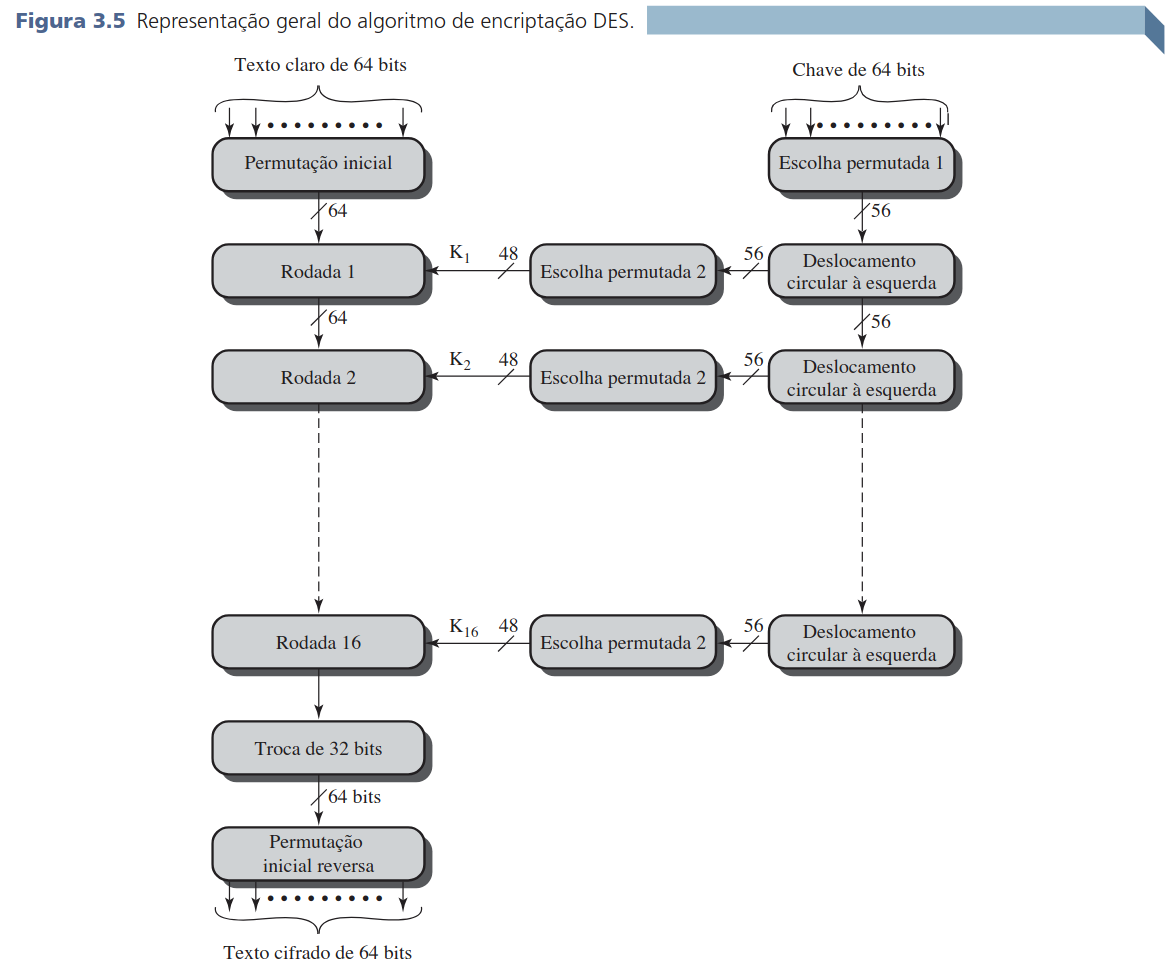
\includegraphics[width=0.6\linewidth]{Figuras/DES-esquema.png}

\end{figure}

\end{frame}

\begin{frame}{Funcionamento DES}
    No esquema de encriptação DES existem duas entradas na função: 
    \textbf{texto claro} (64 bits) e \textbf{chave} (56 bits).

    \vspace{0.3cm}
    \textbf{Processamento do texto claro:}
    \begin{itemize}
        \item \textbf{Permutação Inicial (IP)}: reorganiza os bits do texto claro para produzir a entrada permutada.
        \item \textbf{16 rodadas de função Feistel}: cada rodada envolve permutação e substituição dos bits.
        \item \textbf{Troca das metades esquerda e direita} para gerar a pré-saída.
        \item \textbf{Permutação Final (IP\textsuperscript{-1})}: inverso da permutação inicial, produzindo o texto cifrado de 64 bits.
    \end{itemize}


   
\end{frame}

\begin{frame}{Data Encryption Standard (DES)}
    \begin{itemize}
        \item Cifra de bloco que processa dados em blocos de 64 bits.
        \item Entrada: bloco de texto claro de 64 bits.
        \item Saída: bloco de texto cifrado de 64 bits.
        \item Algoritmo simétrico: mesma chave e mesmo algoritmo para encriptação e decriptação (com pequenas diferenças no escalonamento de chaves).
    \end{itemize}



\end{frame}

\begin{frame}{Esquema detalhado - DES}
\begin{figure}
    \centering
    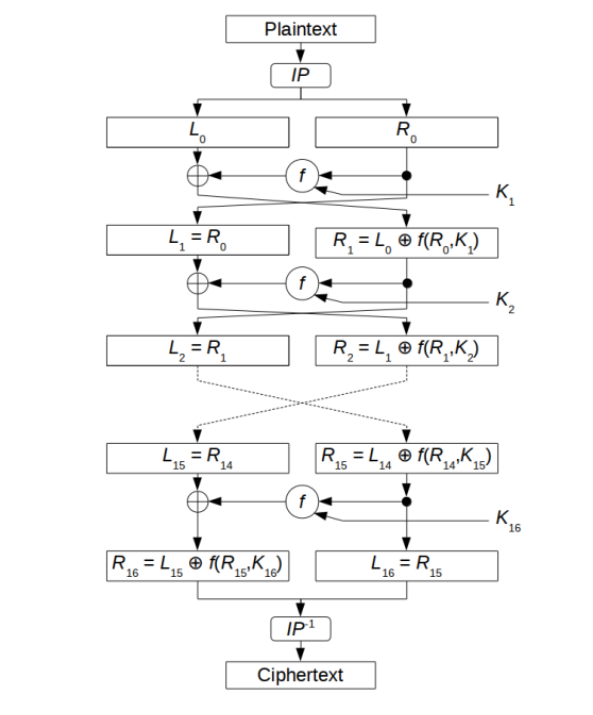
\includegraphics[width=0.45\linewidth]{Figuras/DES-esquema-2.png}

\end{figure}
    
\end{frame}

\begin{frame}{Chaves no DES}
    \begin{itemize}
        \item Comprimento efetivo da chave: 56 bits.
        \item A chave é representada como um número de 64 bits:
        \begin{itemize}
            \item A cada byte, o bit menos significativo é usado para verificação de paridade.
            \item Esses 8 bits de paridade não participam da criptografia.
        \end{itemize}
        \item Existem algumas chaves fracas, mas são facilmente evitáveis.
        \item Toda a segurança do DES depende da chave utilizada.
    \end{itemize}
\end{frame}


\begin{frame}{Funcionamento DES}




    \vspace{0.3cm}
    \textbf{Processamento da chave:}
    \begin{itemize}
        \item Chave de 56 bits passa por uma permutação inicial.
        \item Para cada uma das 16 rodadas, gera-se uma subchave (K\textsubscript{i}) usando:
            \begin{itemize}
                \item Deslocamento circular à esquerda.
                \item Permutação fixa.
            \end{itemize}
        \item Cada rodada utiliza uma subchave diferente, derivada da chave original.
    \end{itemize}

\textbf{Decriptação DES}:
Assim como qualquer cifra de Feistel, a decriptação usa o mesmo algoritmo da encriptação, exceto que a
aplicação das subchaves é invertida. Além disso, as permutações inicial e final são invertidas.
\end{frame}

\begin{frame}{Outline of the DES Algorithm}
    \begin{itemize}
        \item O DES opera sobre blocos de \textbf{64 bits}.
        \item Etapas principais:
        \begin{itemize}
            \item \textbf{Permutação inicial (IP)} sobre o bloco de entrada.
            \item Divisão em duas metades:
            \begin{itemize}
                \item Lado esquerdo (32 bits).
                \item Lado direito (32 bits).
            \end{itemize}
        \end{itemize}
    \end{itemize}


\textbf{Rodadas e Finalização do DES}
    \begin{itemize}
        \item São realizadas \textbf{16 rodadas} de operações idênticas.
        \item Em cada rodada:
        \begin{itemize}
            \item A função $f$ combina dados com subchaves derivadas da chave principal.
        \end{itemize}
        \item Após a 16ª rodada:
        \begin{itemize}
            \item As metades esquerda e direita são reunidas.
            \item Aplica-se a \textbf{permutação final}, inversa da permutação inicial.
        \end{itemize}
    \end{itemize}
\end{frame}

\begin{frame}{DES Round Function $f$}
    \begin{itemize}
        \item Em cada rodada:
        \begin{itemize}
            \item A chave de 56 bits é \textbf{deslocada} e \textbf{reduzida} para 48 bits.
            \item O lado direito (32 bits) é \textbf{expandido} para 48 bits.
            \item Os 48 bits resultantes são combinados com a subchave via \textbf{XOR}.
            \item O resultado passa por \textbf{8 S-boxes}, produzindo 32 bits.
            \item Esses 32 bits sofrem uma \textbf{permutação}.
        \end{itemize}
        \item A saída da função $f$ é combinada com o lado esquerdo via XOR.
        \item Após isso, ocorre a \textbf{troca de metades}.
    \end{itemize}
\textbf{Equações de uma Rodada no DES}
    \[
        L_i = R_{i-1}
    \]
    \[
        R_i = L_{i-1} \oplus f(R_{i-1}, K_i)
    \]
    \begin{itemize}
        \item $L_i, R_i$: metades esquerda e direita no final da rodada $i$.
        \item $K_i$: subchave de 48 bits da rodada $i$.
        \item $f$: função que realiza expansão, XOR, substituições e permutação.
        \item Repetido por \textbf{16 rodadas}.
    \end{itemize}
\end{frame}

\begin{frame}{ Uma rodada do DES}
\begin{figure}
    \centering
    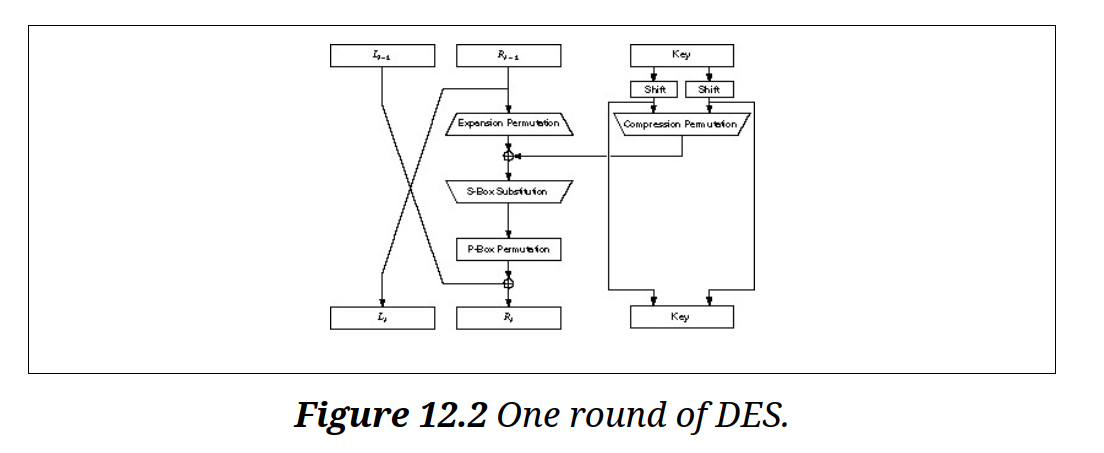
\includegraphics[width=\linewidth]{Figuras/one-round-des.png}

\end{figure}
    
\end{frame}

\begin{frame}{Exemplo do DES}
    Exemplo prático do DES:

    \begin{itemize}
     \item \textbf{Objetivo}: observar os padrões em hexadecimal que surgem de uma etapa para outra, sem necessariamente replicar o cálculo manualmente
   
        \item Texto claro escolhido é um \textbf{palíndromo hexadecimal}.

    \end{itemize}

    \begin{figure}
        \centering
        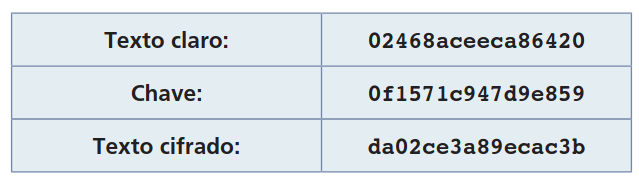
\includegraphics[width=0.5\linewidth]{Figuras/palindromo-hexadecimal-des.png}
    \end{figure}
\end{frame}




\begin{frame}{Exemplo do DES}

\begin{itemize}
        \item Evolução do algoritmo ao longo das rodadas.
        \item Primeira linha: valores de 32 bits das metades esquerda (L) e direita (R) \textbf{após a permutação inicial (IP)}.
        \item Linhas seguintes (1 a 16): resultado após cada rodada, incluindo:
        
        \item Última linha: valores de L e R após a permutação inicial inversa (IP$^{-1}$).
        \item A concatenação desses dois valores gera o \textbf{texto cifrado}.
    \end{itemize}
    \begin{columns}
        \begin{column}{0.48\textwidth}
            \centering
            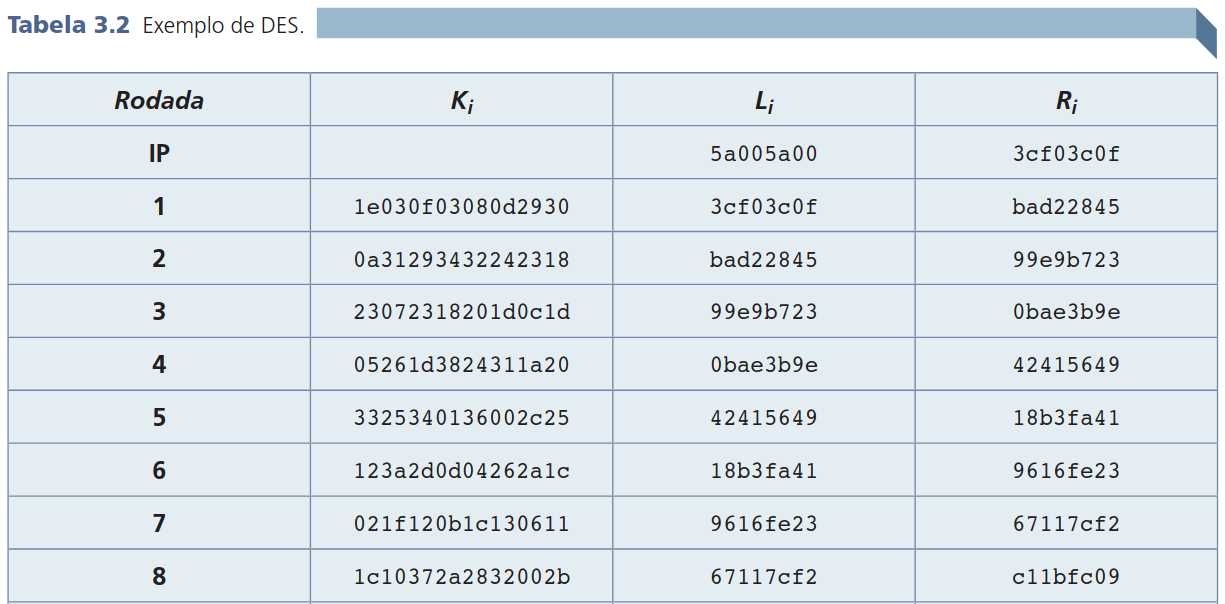
\includegraphics[width=\linewidth]{Figuras/des-lado1.png}

        \end{column}
        \begin{column}{0.48\textwidth}
            \centering
            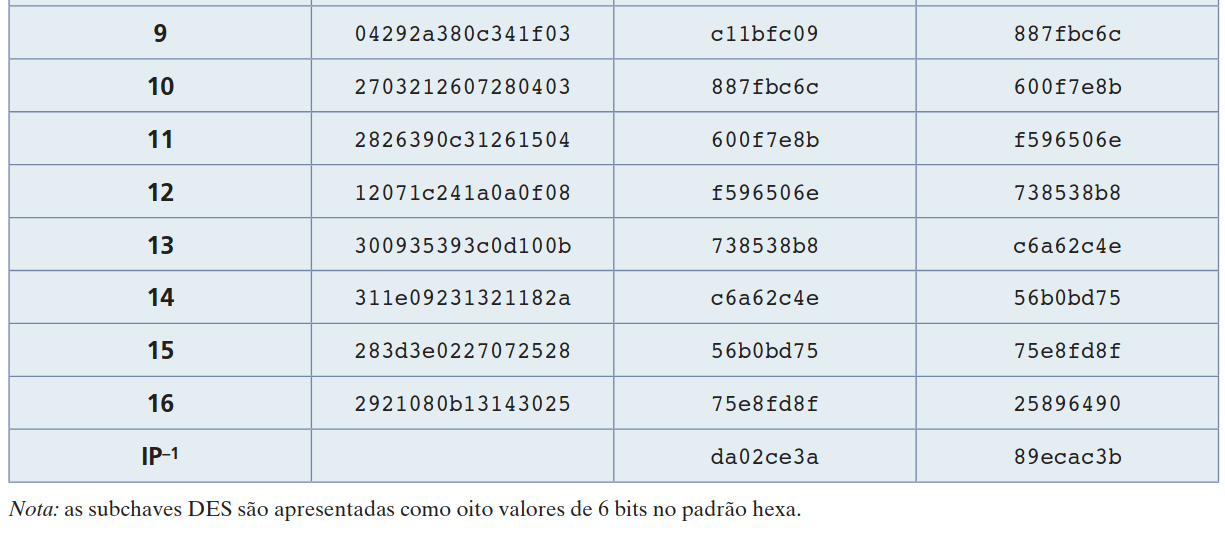
\includegraphics[width=\linewidth]{Figuras/des-lado2.png}
    
        \end{column}
    \end{columns}
\end{frame}

\begin{frame}{Efeito Avalanche}
    \begin{itemize}
        \item Propriedade desejável em algoritmos de encriptação.
        \item Uma pequena mudança no texto claro ou na chave deve causar uma grande alteração no texto cifrado.
        \item \textbf{Objetivo}: Alterar apenas \textbf{um bit} no texto claro ou na chave deve modificar \textbf{muitos bits} no resultado.
        \item \textbf{Resultado esperado}: Caso a mudança fosse pequena, seria possível reduzir o espaço de busca de textos claros ou de chaves.
        \item O efeito avalanche aumenta a segurança, dificultando ataques de análise e padrões previsíveis.
    \end{itemize}
\end{frame}

\begin{frame}{Exemplo do Efeito Avalanche no DES}
    \begin{itemize}
        \item Texto claro inicial  modificado no 4º bit.
        \item Tabela de acompanhamento mostra:
        \begin{itemize}
            \item Coluna 1: rodadas do algoritmo.
            \item Coluna 2: valores intermediários de 64 bits no final de cada rodada.
            \item Coluna 3: número de bits diferentes entre os dois textos.
        \end{itemize}
        \item Após apenas 3 rodadas: diferença de \textbf{18 bits}.
        \item Texto cifrado final: diferença de \textbf{32 bits}.
        \item Demonstra claramente o \textbf{efeito avalanche} do DES.
    \end{itemize}


    
\end{frame}


\begin{frame}{Exemplo do Efeito Avalanche no DES}


\centering
    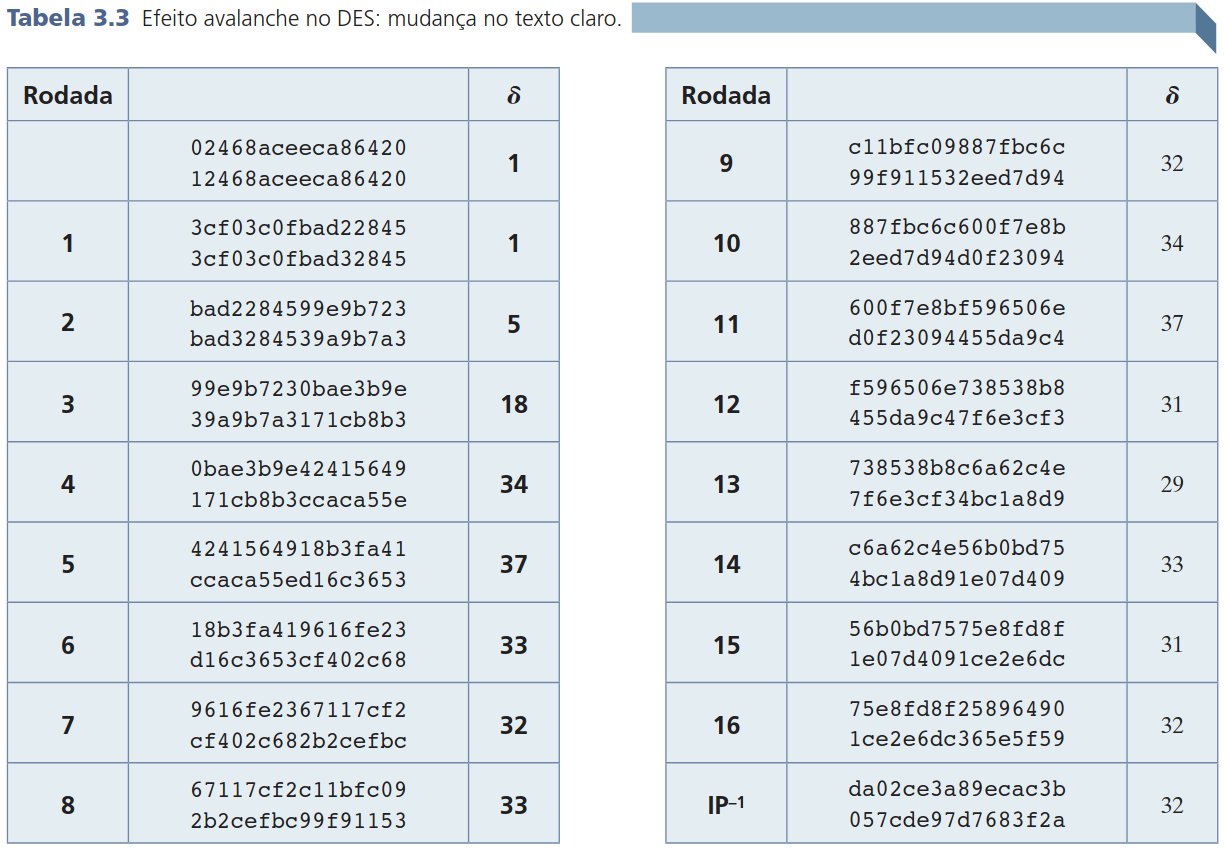
\includegraphics[width=0.7\linewidth]{Figuras/des-efeito-avalanche.png}
    
\end{frame}

\begin{frame}{Efeito Avalanche com Alteração da Chave}
\textbf{Experimento}: Texto claro mantido constante mas com duas chaves utilizadas:
        \begin{itemize}
            \item Chave original modificada \textbf{com diferença no 4º bit}
        \end{itemize}
\textbf{Resultados}:
        \begin{itemize}
            \item Diferença significativa no texto cifrado final — cerca de metade dos bits são diferentes.
            \item O efeito avalanche já aparece após poucas rodadas do DES.
        \end{itemize}
 \textbf{Demonstra}: Robustez do algoritmo contra pequenas alterações na chave.

\end{frame}

\begin{frame}{Exemplo do Efeito Avalanche no DES - Mudança na chave}


\centering
    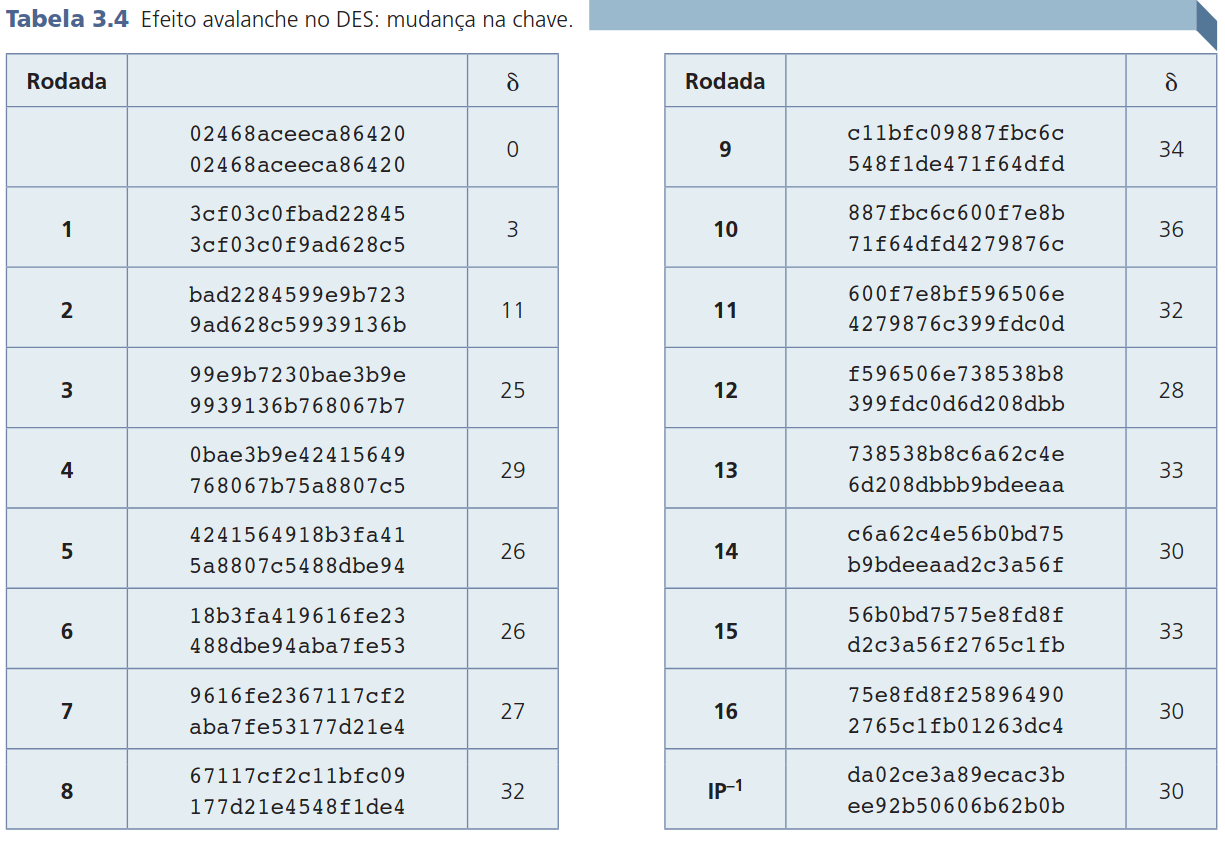
\includegraphics[width=0.7\linewidth]{Figuras/des-efeito-avalanche-chave.png}
    
\end{frame}

\begin{frame}{A Força do DES}
    \begin{itemize}
        \item Desde sua adoção como padrão federal, surgiram preocupações sobre a segurança do DES.
        \item Principais áreas de preocupação:
        \begin{itemize}
            \item \textbf{Tamanho da chave}: 56 bits pode ser vulnerável a ataques de força bruta.
            \item \textbf{Natureza do algoritmo}: estrutura e procedimentos internos do DES podem influenciar sua resistência a ataques criptográficos.
        \end{itemize}
        \item Essas questões motivaram o desenvolvimento de algoritmos mais seguros, como o Triple DES (3DES) e o AES.
    \end{itemize}
\end{frame}

\begin{frame}{Uso de Chaves de 56 Bits no DES}
    \begin{itemize}
        \item Chave de 56 bits → $2^{56} \approx 7,2 \times 10^{16}$ chaves possíveis.
        \item Ataque de força bruta \textbf{pareceria} impraticável:
        \begin{itemize}
            \item Pesquisando metade do espaço de chaves
            \item Uma máquina realizando 1 encriptação por microssegundo levaria mais de 1000 anos.
        \end{itemize}
        \item No entanto, Diffie e Hellman (1977) propuseram tecnologia paralela:
        \begin{itemize}
            \item Máquina com 1 milhão de dispositivos, cada um realizando 1 encriptação/µs.
            \item Tempo médio de busca: cerca de 10 horas.
            \item Custo estimado: US\$ 20 milhões (em 1977).
        \end{itemize}
        \item Demonstra que, apesar do tamanho da chave, o DES não é invulnerável a ataques especializados.
    \end{itemize}
\end{frame}

\begin{frame}{Impacto da Tecnologia Moderna na Segurança do DES}
    \begin{itemize}
        \item Atualmente, nem é necessário hardware especial para ataques de força bruta contra o DES.
        \item Processadores comerciais modernos já oferecem velocidades que ameaçam a segurança do DES:
        \begin{itemize}
            \item Computadores multicore atuais: ~ $10^9$ combinações de chaves por segundo [SEAG08].
            \item Testes em máquinas Intel multicore: ~ $5 \times 10^8$ encriptações por segundo [BASU12].
            \item Supercomputadores contemporâneos: ~ $10^{13}$ encriptações por segundo.
        \end{itemize}
        \item Instruções de hardware recentes para AES também aceleram operações criptográficas, mostrando que ataques de força bruta se tornam cada vez mais viáveis.
        \item Conclusão: o DES, com chave de 56 bits, é vulnerável diante da tecnologia atual.
    \end{itemize}
\end{frame}

\begin{frame}{Força Bruta e Tamanho da Chave}
    \begin{itemize}
        \item Tabela 3.5 mostra o tempo necessário para ataques de força bruta em diferentes tamanhos de chave.
        \item Exemplos:
        \begin{itemize}
            \item Um único PC moderno pode quebrar o DES (56 bits) em ~1 ano.
            \item Vários PCs em paralelo reduzem drasticamente o tempo.
            \item Supercomputadores contemporâneos: ~1 hora para descobrir a chave do DES.
        \end{itemize}
        \item Chaves de 128 bits ou mais são efetivamente inquebráveis por força bruta:
        \begin{itemize}
            \item Mesmo com aceleração de $10^{12}$ vezes, ainda seriam necessários ~100 mil anos.
        \end{itemize}
        \item Alternativas mais seguras ao DES: \textbf{AES} e \textbf{Triple DES}
    \end{itemize}
\end{frame}

\begin{frame}{Exemplo do Efeito Avalanche no DES - Mudança na chave}


\centering
    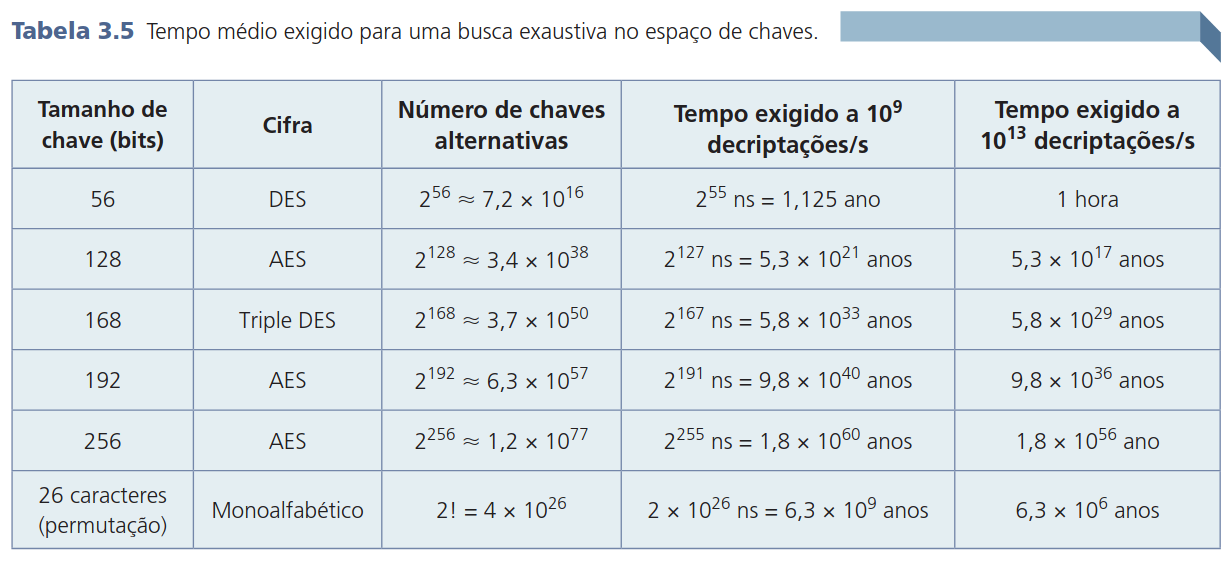
\includegraphics[width=0.9\linewidth]{Figuras/tempo-para-quebrar.png}
    
\end{frame}

\begin{frame}{Resumo - Projeto de cifra de bloco}
\textbf{Número de Rodadas no DES}
    \begin{itemize}
        \item Maior número de rodadas → mais difícil a criptoanálise, mesmo se a função $F$ for relativamente fraca.
        \item Critério de projeto: número de rodadas suficiente para que criptoanálises conhecidas exijam mais esforço do que um ataque de força bruta.
        \item No DES:
        \begin{itemize}
            \item 16 rodadas
            \item Criptoanálise diferencial: $2^{55,1}$ operações
            \item Força bruta: $2^{55}$ operações
            \item Se houvesse 15 ou menos rodadas, criptoanálise diferencial exigiria menos esforço que a força bruta.
        \end{itemize}
        \item Critério facilita comparar a força de diferentes algoritmos.
        \item Sem descobertas revolucionárias em criptoanálise, a força de um algoritmo que satisfaz este critério é julgada principalmente pelo tamanho da chave.
    \end{itemize}


    
\end{frame}

\begin{frame}{Resumo - Projeto de cifra de bloco}

\textbf{Projeto da Função F no DES}
    \begin{itemize}
        \item A função $F$ é o núcleo da cifra de bloco de Feistel e é responsável pela \textbf{confusão}.
        \item Critérios importantes para o projeto de $F$:
        \begin{itemize}
            \item \textbf{Não linearidade}: quanto menos linear, mais difícil a criptoanálise.
            \item \textbf{Efeito avalanche}: mudança em 1 bit da entrada altera muitos bits da saída.
            \item \textbf{Strict Avalanche Criterion (SAC)} [WEBS86]:
            \begin{itemize}
                \item Qualquer bit de saída muda com probabilidade 1/2 quando qualquer bit de entrada é invertido.
                \item Originalmente definido para S-boxes, mas aplicável à função $F$ como um todo.
            \end{itemize}
            \item \textbf{Bit Independence Criterion (BIC)} [WEBS86]:
            \begin{itemize}
                \item Bits de saída mudam independentemente quando qualquer bit de entrada é invertido.
            \end{itemize}
        \end{itemize}
        \item Aplicar SAC e BIC fortalece a eficácia da função de confusão e aumenta a segurança do algoritmo.
    \end{itemize}
\end{frame}

\begin{frame}{Resumo - Projeto de cifra de bloco}

\textbf{Algoritmo de Escalonamento de Chave}
    \begin{itemize}
        \item Em cifras de bloco de Feistel, a chave principal é usada para gerar uma \textbf{subchave} para cada rodada.
        \item Objetivo do escalonamento de chave:
        \begin{itemize}
            \item Maximizar a dificuldade de deduzir subchaves individuais.
            \item Tornar mais difícil recuperar a chave principal a partir das subchaves.
        \end{itemize}
        \item Não existe, até o momento, um princípio geral universalmente aceito para o projeto do algoritmo de escalonamento de chaves.
        \item O cuidado no escalonamento é crucial para garantir a segurança global do algoritmo.
    \end{itemize}
\end{frame}

\begin{frame}{Triple DES (3DES)}
    \begin{itemize}
        \item Primeiro padronizado em 1985 pela ANSI para aplicações financeiras (X9.17).
        \item Incorporado ao DES como parte do padrão FIPS 46-3 em 1999.
        \item Utiliza \textbf{três chaves} e três execuções do algoritmo DES.
        \item Sequência de operação: \textbf{Encrypt-Decrypt-Encrypt (EDE)}:
        \[
            C = E(K_3, D(K_2, E(K_1, P)))
        \]
        \begin{itemize}
            \item $C$ = texto cifrado
            \item $P$ = texto claro
            \item $K_1, K_2, K_3$ = chaves
        \end{itemize}
        \item A abordagem EDE garante compatibilidade com DES original quando $K_1 = K_2 = K_3$.
    \end{itemize}
\end{frame}

\begin{frame}{Diretrizes do FIPS 46-3 para 3DES}
    \begin{itemize}
        \item 3DES é o algoritmo de cifra simétrica aprovado pelo FIPS para uso corrente.
        \item O DES original (chave de 56 bits) é permitido apenas para sistemas legados.
        \item Novas aquisições de sistemas devem suportar 3DES.
        \item Organizações governamentais com sistemas DES legados são incentivadas a migrar para 3DES.
        \item Espera-se que 3DES e AES coexistam como algoritmos aprovados pelo FIPS, permitindo uma transição gradual para AES.
    \end{itemize}
\end{frame}


\begin{frame}{Exemplo do Efeito Avalanche no DES - Mudança na chave}


\centering
    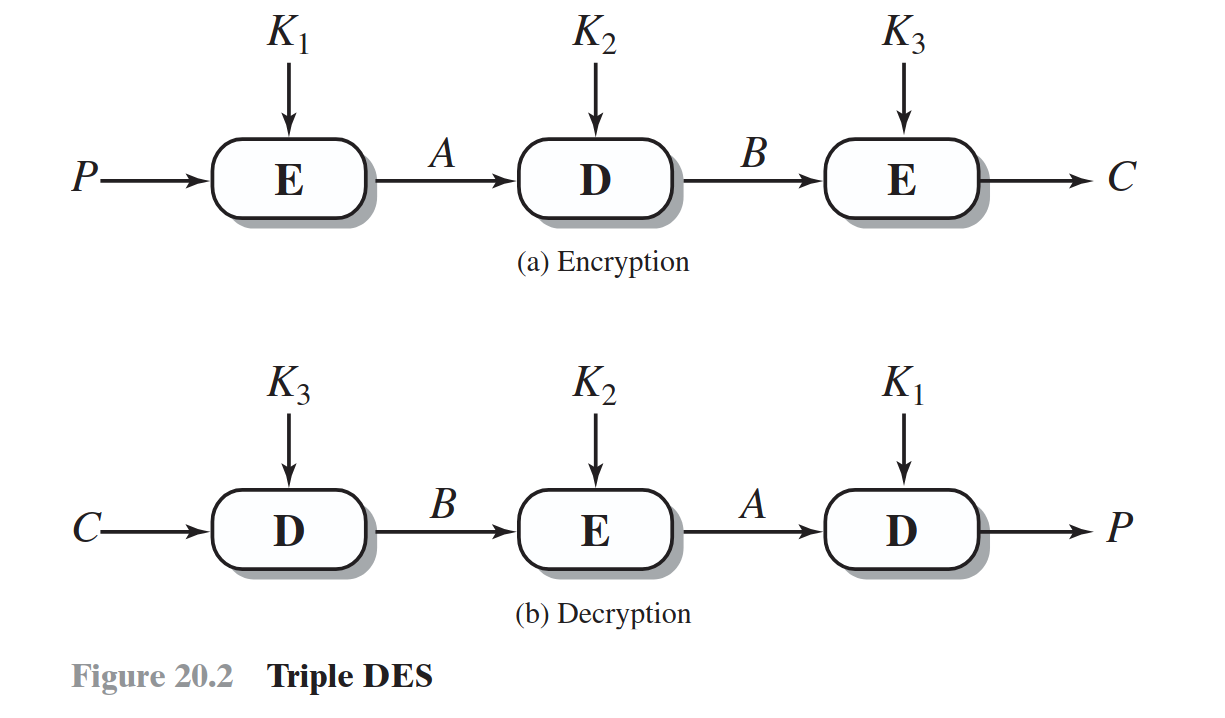
\includegraphics[width=0.9\linewidth]{Figuras/3des-ede.png}
    
\end{frame}

\begin{frame}{Compatibilidade do 3DES com DES}
    \begin{itemize}
        \item Quando as três chaves são iguais ($K_1 = K_2 = K_3$), temos:
        \[
            C = E(K_1, D(K_1, E(K_1, P))) = E(K, P)
        \]
        \item A operação do meio $D(K_1, E(K_1, P))$ se anula, resultando apenas na cifra DES original.
        \item Importância:
        \begin{itemize}
            \item Permite que dados cifrados com DES possam ser decifrados por um sistema 3DES configurado em modo compatível.
            \item Sistemas antigos que usam DES podem processar dados cifrados por 3DES no modo compatível.
        \end{itemize}
        \item Essa retrocompatibilidade facilitou a adoção do 3DES sem necessidade de substituir todos os sistemas legados.
    \end{itemize}
\end{frame}


\begin{frame}{Chaves e Criptografia no 3DES}
    \begin{itemize}
        \item O uso da decriptação na segunda etapa do 3DES não tem significado criptográfico;  
              sua vantagem é permitir compatibilidade com o DES original:
        \[
            C = E(K_1, D(K_1, E(K_1, P))) = E(K, P)
        \]
        \item Com três chaves distintas ($K_1, K_2, K_3$), o 3DES possui \textbf{168 bits efetivos de chave}.
        \item É possível usar apenas duas chaves ($K_1 = K_3$), resultando em uma chave efetiva de \textbf{112 bits}.
        \item O padrão FIPS 46-3 fornece diretrizes formais para a utilização do 3DES com estas configurações.
    \end{itemize}
\end{frame}

\begin{frame}{Chaves e Criptografia no 3DES}
    \begin{itemize}
        \item O uso da decriptação na segunda etapa do 3DES não tem significado criptográfico;  
              sua vantagem é permitir compatibilidade com o DES original:
        \[
            C = E(K_1, D(K_1, E(K_1, P))) = E(K, P)
        \]
        \item Com três chaves distintas ($K_1, K_2, K_3$), o 3DES possui \textbf{168 bits efetivos de chave}.
        \item É possível usar apenas duas chaves ($K_1 = K_3$), resultando em uma chave efetiva de \textbf{112 bits}.
        \item O padrão FIPS 46-3 fornece diretrizes formais para a utilização do 3DES com estas configurações.
    \end{itemize}
\end{frame}

\begin{frame}{Advanced Encryption Standard (AES) e Rijndael}
    \begin{itemize}
        \item Publicado pelo \textbf{NIST} em 2001 como padrão de cifra simétrica de bloco.
        \item Substitui o DES em diversas aplicações, oferecendo maior segurança e eficiência.
        \item AES é mais complexo que cifras de chave pública (ex.: RSA), sendo difícil de explicar de forma simplificada.
        \item Em 2000, o NIST selecionou a família de cifras de bloco \textbf{Rijndael} como vencedora do concurso AES.
                \item \textbf{Rijndael}: cifra de bloco escolhida como AES pelo NIST. 
                \item \textbf{AES não usa Cifra de Feistel}
 
               \item Três variantes especificadas: AES-128; AES-192; AES-256
    \end{itemize}
\end{frame}

\begin{frame}{Tipos AES}


\centering
    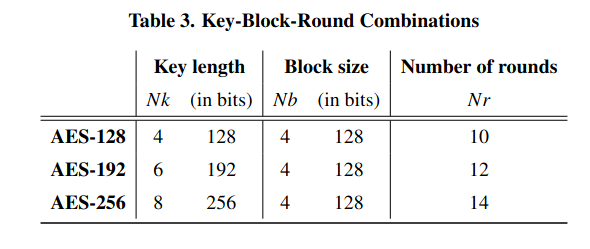
\includegraphics[width=0.9\linewidth]{Figuras/tipos-aes.png}
    
\end{frame}

\begin{frame}{Diferenças entre AES-128, AES-192 e AES-256}
    \begin{itemize}
        \item As três variantes diferem em três aspectos principais:
        \begin{enumerate}
            \item \textbf{Comprimento da chave} (128, 192 ou 256 bits).
            \item \textbf{Número de rodadas (Nr)}, que determina o tamanho do key schedule.
            \item \textbf{Especificação da recursão em KEY EXPANSION()}.
        \end{enumerate}
        \item Para cada algoritmo:
        \begin{itemize}
            \item \textbf{Nr}: número de rodadas.
            \item \textbf{Nk}: número de palavras da chave.
            \item \textbf{Nb}: número de palavras do estado; no padrão AES, \textbf{Nb = 4}.
        \end{itemize}
        \item Somente essas configurações de Rijndael estão conformes com o padrão AES.

        \item  \href{https://csrc.nist.gov/pubs/fips/197/final}{\textcolor{blue}{Veja a especificação FIPS 197 do AES}}
    \end{itemize}

   
\end{frame}

\begin{frame}{AES também suporta vários modos}

\textbf{Exemplos de modos de operação:}
\begin{itemize}
    \item AES-ECB (Electronic Codebook)
    \item AES-CBC (Cipher Block Chaining)
    \item AES-CTR (Counter Mode)
    \item AES-GCM (Galois/Counter Mode)
    \item \href{https://ieeexplore.ieee.org/stamp/stamp.jsp?arnumber=7946655&casa_token=xII8ag99IPsAAAAA:p362qc3e09WXdTSoT4jOMXCsgCvsdOqc6QuPWiYXum-XcZB1BVzeB9OkdaigwbC5qQYOcDscAw}{\textcolor{blue}{Artigo: A Comparative Analysis of AES Common Modes of Operation}}
    \item \href{https://ciit.finki.ukim.mk/data/papers/10CiiT/10CiiT-46.pdf}{\textcolor{blue}{Artigo: MODES OF OPERATION OF THE AES ALGORITHM}}
\end{itemize}
    
\end{frame}

\begin{frame}{Electronic Code Book (ECB) – Considerações}
    \begin{itemize}
        \item O modo ECB divide a mensagem em blocos ($P_1, P_2, \dots, P_N$) e cifra cada bloco separadamente com a mesma chave $K$.
        \item Se a mensagem não preencher o último bloco, ele é completado com \textit{padding}.
        \item Vantagem: erros em um bloco não se propagam para os outros, permitindo decifrar blocos não corrompidos.
        \item Desvantagem: a criptografia é determinística; blocos de texto claro idênticos produzem blocos cifrados idênticos.
        \item Problemas adicionais:
        \begin{itemize}
            \item Blocos idênticos ou mensagens com início igual são facilmente reconhecíveis.
            \item A ordem dos blocos cifrados pode ser alterada sem que o receptor perceba.
        \end{itemize}
        \item Conclusão: não recomendado para dados maiores que um bloco; alguns autores desaconselham completamente seu uso.
    \end{itemize}
\end{frame}

\begin{frame}{Modo ECB}


\centering
    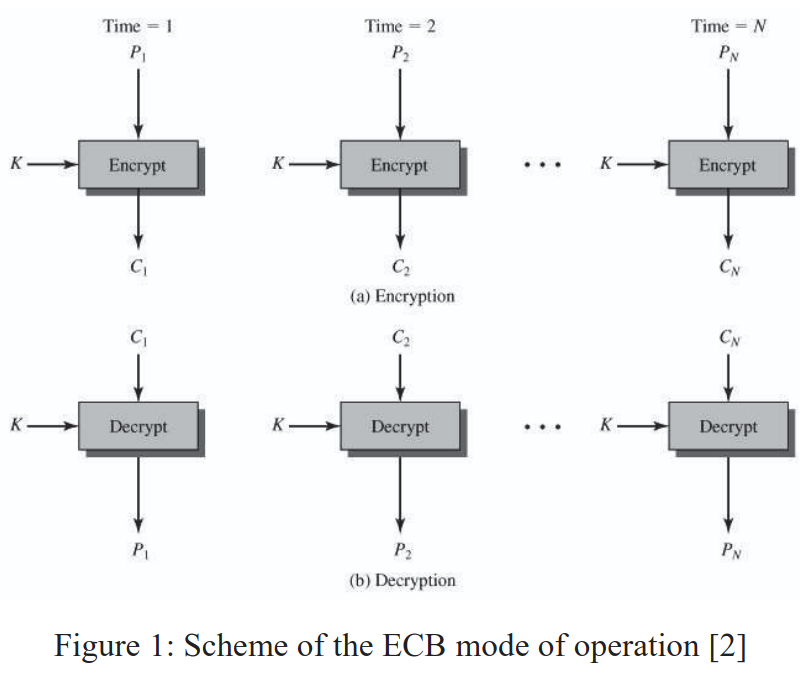
\includegraphics[width=0.6\linewidth]{Figuras/aes-modo-ecb.png}
    
\end{frame}

\begin{frame}{Cipher Block Chaining (CBC) – Considerações}
    \begin{itemize}
        \item O modo CBC resolve o problema do ECB, reduzindo padrões repetidos no texto cifrado.
        \item Cada bloco de texto claro é XORado com o bloco cifrado anterior antes da encriptação.
        \item O primeiro bloco de texto claro é XORado com um \textit{initialization vector} (IV).
        \item Benefício: mensagens longas com padrões repetidos podem ser tratadas de forma mais segura.
        \item Resultados de cifras distintas: mesmo texto claro cifrado múltiplas vezes gera diferentes textos cifrados devido ao IV.
        \item Desvantagem: requer mais tempo de processamento que o ECB devido ao encadeamento.
        \item Pode ser sincronizado para evitar propagação de erros causados por ruído no canal.
        \item O CBC não suporta paralelismo (\textbf{diferentemente do ECB)}
    \end{itemize}
\end{frame}

\begin{frame}{Modo CBC}


\centering
    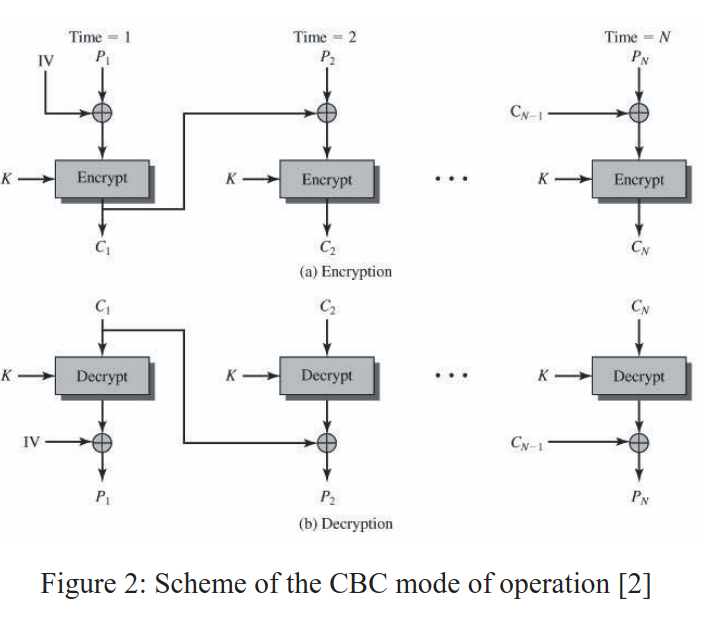
\includegraphics[width=0.6\linewidth]{Figuras/aes-modo-cbc.png}
    
\end{frame}

\begin{frame}{Counter Mode (CTR)}
    \begin{itemize}
        \item Usa um contador como vetor de inicialização (IV), com tamanho igual ao do bloco.
        \item Cada bloco de texto claro é XORado com a saída da cifra aplicada ao contador.
        \item Não há necessidade de \textit{padding} no último bloco.
        \item Os blocos são independentes, sem propagação de erro entre eles.
        \item Suporta paralelismo e pré-processamento, acelerando cifragem/decifragem.
        \item As operações de encriptação e decriptação são idênticas.
        \item É fundamental não reutilizar o mesmo contador com a mesma chave, sob risco de quebra completa da confidencialidade.
        \item Normalmente, o contador é inicializado com um valor único (ex.: 96 bits aleatórios + 32 bits incrementais).
        \item A chave deve ser trocada após $2^{n/2}$ blocos (onde $n$ é o tamanho do bloco).
        \item Considerado um dos modos mais seguros e eficientes para AES.
    \end{itemize}
\end{frame}

\begin{frame}{Modo CTR}


\centering
    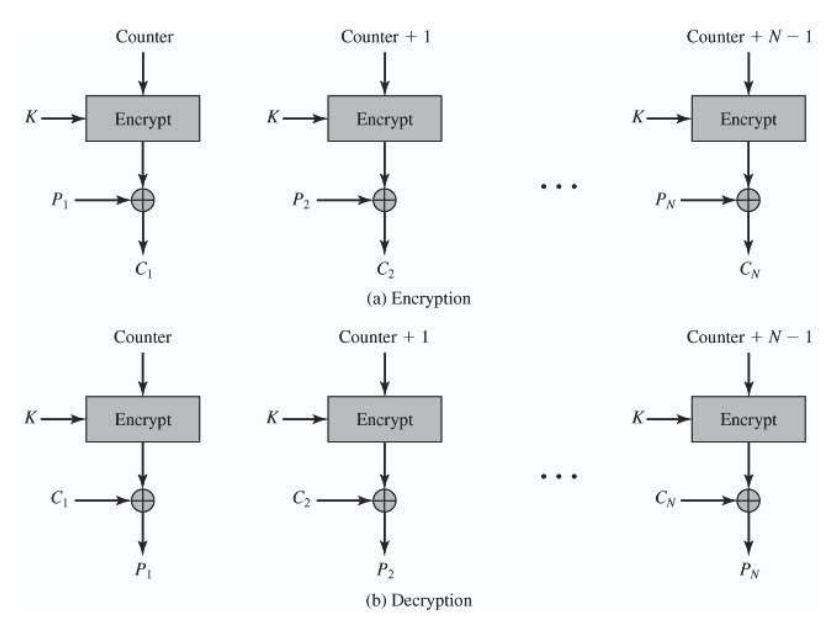
\includegraphics[width=0.6\linewidth]{Figuras/aes-modo-ctr.png}
    
\end{frame}

\begin{frame}{AES -- Galois/Counter Mode (GCM)}
    \begin{itemize}
        \item GCM combina duas funções: 
        \begin{itemize}
            \item \textbf{Autenticação}: cálculo de um \textit{tag} de integridade.
            \item \textbf{Confidencialidade}: criptografia no modo \textit{Counter}.
        \end{itemize}
        \item O processo de confidencialidade é baseado no modo CTR (\textit{Counter Mode}).
        \item A autenticação é realizada pela função \textbf{GHASH}, que usa multiplicações em $\text{GF}(2^{128})$.
        \begin{itemize}
            \item \(GF(2^{128})\) é o campo de Galois com 128 bits: cada bloco de 128 bits é tratado como um polinômio de grau \(\leq 127\) com coeficientes 0 ou 1; a soma é XOR e a multiplicação é feita módulo 
\[
p(x) = x^{128}+x^7+x^2+x+1.
\]
        \end{itemize}
        \item O \textit{hash subkey} $H$ é obtido aplicando AES sobre o bloco nulo.
        \item O \textit{tag} de autenticação $T$ é gerado a partir dos dados confidenciais e dos dados adicionais autenticados (AAD).
        \item Na decriptação autenticada, o \textit{tag} é verificado para garantir integridade e autenticidade.
        \item \href{https://ieeexplore.ieee.org/abstract/document/5953585?casa_token=4XfQGwEHfSEAAAAA:RZKOvTWEOaYpC0nIW8kEB8omke-XhdiG9iwkC4OEsp1yMXiZ6lIv6ckx9g_CffSJiCGgF9QCEg}{\textcolor{blue}{Artigo: Modo GCM}}
    \end{itemize}
\end{frame}

\begin{frame}{Modo GCM}


\centering
    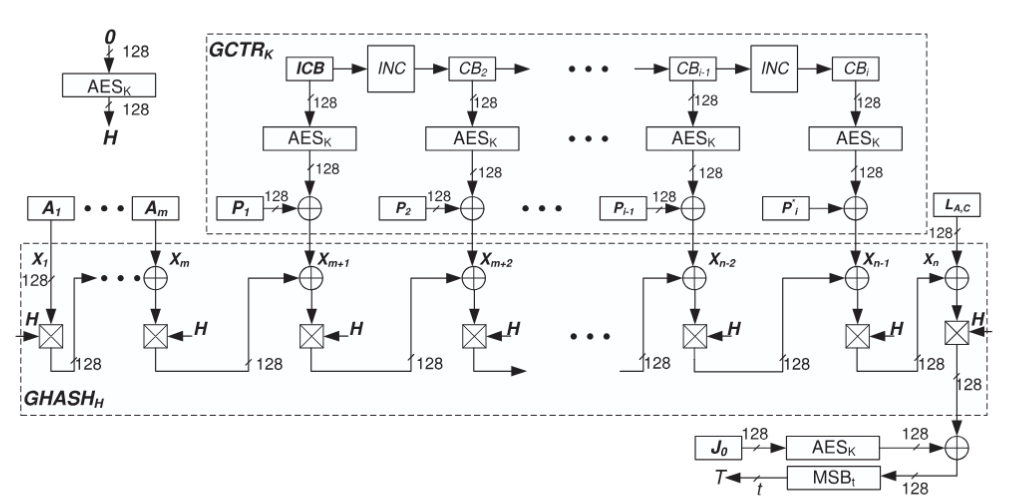
\includegraphics[width=0.8\linewidth]{Figuras/aes-modo-gcm.png}
    
\end{frame}

\begin{frame}{AES-GCM: Campo de Galois e GHASH}
\begin{itemize}
    \item O GCM usa o campo finito \(GF(2^{128})\) para autenticação.
    \item Cada bloco de 128 bits é tratado como um polinômio de grau até 127:
    \[
        b_0 + b_1 x + b_2 x^2 + \dots + b_{127} x^{127}, \quad b_i \in \{0,1\}
    \]
    \item A chave de hash \(H\) é gerada cifrando um bloco de zeros com AES.
    \item O GHASH combina cada bloco de dados ou AAD com \(H\) assim:
    \[
        X_i = (X_{i-1} \oplus B_i) \cdot H \mod p(x)
    \]
    \item O polinômio irreducível usado é fixo pelo padrão NIST:
    \[
        p(x) = x^{128} + x^7 + x^2 + x + 1
    \]
\end{itemize}
\end{frame}

\begin{frame}{Fluxo de autenticação no AES-GCM (GHASH)}
O fluxo de autenticação no AES-GCM (GHASH) funciona assim:

\begin{enumerate}
    \item Pega o acumulador do bloco anterior $X$ (ou zero no primeiro bloco).
    \item Faz XOR com o bloco atual da mensagem $P$.
    \item Multiplica o resultado pelo $H$, que é a chave de hash obtida cifrando um bloco de zeros com AES.
    \item Reduz módulo o polinômio
    \[
        p(x) = x^{128} + x^7 + x^2 + x + 1
    \]
    para manter 128 bits.
\end{enumerate}

Ou seja, cada passo é:
\[
X_i = ((X_{i-1} \oplus P_i) \cdot H) \bmod p(x)
\]

\begin{itemize}
    \item O XOR encadeia os blocos e mistura os dados.
    \item O módulo garante que o resultado continue com 128 bits, pronto para o próximo bloco ou para gerar a Tag final.
\end{itemize}
\end{frame}
